\chapter{Machine Learning Fundamentals}
As machine learning techniques will be used for the classification of individual tap locations on a smartphone touchscreen, the following chapter will give a brief overview of the fundamental concepts evolving around statistical learning. Individual categories of learning algorithms will be discussed followed by two supervised-learning algorithms, namly Support Vector Machines and Neural Networks.

\section{Overview and Definition}

Ever since computers were invented, there has been a desire to enable them to learn \cite{samuel2000some}. This desire has grown into the field of machine learning which seeks to answer questions on how to build systems that automatically improve with experience. Machine learning covers a set of methods and algorithms designed to accomplish tasks where conventional hard-coded routines have brought insufficient results \cite{mitchell2006discipline}.

The goal of a machine learning algorithm is to learn a function f that is able to predict sensible output values $y \in Y$ give input values $x \in X$:

\begin{equation}
  f: X \rightarrow Y
\end{equation}

Solving this problem is hard as the amount of input values used for learning this function is typically smaller in size than the unseen input values on to which f is applied to. Therefore, the challenge lies in finding a function that generalizes to unseen input values without simply remembering the seen inputs.

Mathematically, machine learning problems are formalized as optimization problems of an objective function which indicates the quality of the functional mapping between $X$ and $Y$. This problem can either be a maximization or minimization problem. If we speak of the latter, the objective function is referred to as the \textit{error function}.

There are four main categories of machine learning methods to be found in literature which all differ in their approach to learn the function f and in respect to the amount of training samples available \cite{Duda:2000:PC:954544, Marsland:2009:MLA:1571643}. These categories consist of \textit{supervised learning}, \textit{unsupervised learning}, \textit{reinforcement learning} and \textit{evolutionary learning}. As the task at hand refers to a supervised learning problem, supervised learning will be outlined in the following.

\section{Supervised Learning}

%%REAL
Supervised learning refers to the case where $N$ samples are given from $X \times Y$, called the training data set  $T = \{ x^{(i)}, y^{(i)} | i \in \{i=1 \dots N\} \}$. The training data is assumed to consist of approximate samples of a target function $F: X \rightarrow Y$, that is be learned by the learning algorithm. The data samples $x^{(i)} \in X$ are called input \textit{features} whereas $y^{(i)} \in Y$ correspond to the so-called \textit{labels}. If Y consists of discrete labels the learning problem corresponds to a classification task whereas if Y is on a continuous scale the problem refers to a regression task (see \cite{Marsland:2009:MLA:1571643}).

Practical applications of supervised learning are image recognition \cite{simonyan2014very, lecun1990handwritten}, e-mail spam filtering \cite{guzella2009review} or network anomaly detection \cite{lee2010uncovering}. However, these are just a small subset of what can be accomplished so far.

Presumably the most widely known machine learning techniques belong to this category, such as the Support Vector Machines (SVMs), Artificial Neural Networks, Bayesian Statistics, Random Forests and Decision Trees \cite{Duda:2000:PC:954544}.

\section{Bias-Variance Trade-off}
The error of a supervised learning algorithm can be decomposed into three components being bias, variance and noise (see \cite{efron_hastie_2016}):

\begin{equation}
  \text{error} = (\text{bias})^2 + \text{variance} + \text{noise}
\end{equation}

%In general, more flexible statistical methods have higher variance.
The \textit{Variance} refers to the amount of which $f$ adapts to the variations in the training data set. Models with a high variance have a tendency to learn minor relations irrespective of the real signal of the input values and are therefore prone to \textit{overfitting} the training examples. This phenomenon applies to very flexible models such as a complex artificial neural network. On the other hand, \textit{bias} is the model's tendency to consistently learn the wrong things from the training examples as it can not take all the information into account. This refers to a too simple model \textit{underfitting} the training examples. An example of high bias would be a linear method such as linear regression trying to map a non-linear function. Finally, the \textit{noise} is the irreducible error of the data distribution (see \cite{James:2014:ISL:2517747}.

As the goal is to minimize the error function, there is always a trade-off between bias and variance with very flexible models having low bias and high variance, and rigid models having high bias and low variance. Therefore, the model with the ideal predictive capability is the one that leads to the best balance between bias and variance \cite{Duda:2000:PC:954544}.

\section{Support Vector Machines}
The SVM is a non-linear kernel based extension of the so-called maximum margin classifier. Originating from binary classification problems, were $y \in \{1, -1\}$, the general idea of a maximum margin classifier is to find a separating hyperplane in the p-dimensional feature space. 

This hyperplane separates the training examples leading to a maximum distance between the observations of the two classes. This distance is referred to as margin $M$ measuring the smallest distance of a training observation towards the defined hyperplane. Mathematically, the support vector classifier can be described as following optimization problem \cite{James:2014:ISL:2517747}:
\begin{eqnarray}
  & \max_{\beta, \epsilon} M \\
  & \textrm{subject to} \sum_{s=1}^{p} \beta^2_s = 1 \\
  g(x_{i}) &= y_i(\beta_0, \beta_1 x_1, \dots \beta_p x_p) \geq M(1 - \epsilon) \\
  & \epsilon \geq 0, \sum_{i=1}^n \epsilon_i \leq C
\end{eqnarray}

The objective of this optimization problem is to maximize the margin $M$ while choosing appropriate vector parameters $\beta$ and $\epsilon$. In this context, the parameter vector $\beta$ contains the coefficients of the hyperplane whereas the vector $\epsilon$ includes so-called slack variables that account for instances which are located on the wrong side of the margin and the hyperplane. These can be expressed as follows assuming that M is positive \cite{James:2014:ISL:2517747}:
\begin{equation}
  \epsilon_i =
  \begin{cases}
    0 & g(x_i) \geq M \\
    > 0 & M < g(x_i) < 0 \\
    > 1 & g(x_i) > 0 
  \end{cases}
\end{equation}

The hyperparameter C allows for a certain sum of $\epsilon_i$ observations to be on the wrong side of the margin or hyperplane, respectively \cite{James:2014:ISL:2517747}. C manages the bias-variance trade-off, since a low C tries to find a maximum margin hyperplane that separates the two classes, resulting in a low bias classifier for the available data set, but in a high variance classifier for test data. Subsequently, allowing a high C results in a high bias classifier that widens the margin, introducing more violations $\epsilon_i$ and reducing the variance of the classifier. Futhermore, C also controls the number of considered support vectors in dependence of the margin width (see \cite{efron_hastie_2016}).

Extending the support vector classifier to non-linear decision boundaries brings us to the SVM. Instead of extending the predictor space using higher order polynomials and interactions, SVM uses the so called ``kernel trick'' \cite{efron_hastie_2016} resulting in the optimization problem to be rewritten as follows:

\begin{equation}
  \hat f(x) = \beta_0 + \sum_{i \in S} \alpha_i \langle x, x_i \rangle \,
\end{equation}

where $i \in S$ defines the subset of support vectors and $\langle x, x_i \rangle$ is the dot product of all pairs in the support vector. Thus, the parameters $\beta_0$ and $\sum_{i \in S}$ can be estimated with the help of least squares by computing the inner products of each pair in the support vector \cite{efron_hastie_2016}. The expression in $\langle x, x_i \rangle$ can be generalized by a kernel function
\begin{equation} \label{eqn:kernel}
  K(x_i,x_{i'}) = \sum_{s=1}^{p} x_{is} x_{i's}
\end{equation}
indicating the linear kernel that quantifies the distance between each pair in the data set \cite{James:2014:ISL:2517747}. Accordingly, the equation above can be rewritten as
\begin{equation}
  \hat f(x) = \beta_0 + \sum_{i \in S} \alpha_i K(x, x_i)
\end{equation}
but in spite of restricting $K(\cdot, \cdot)$ to \ref{eqn:kernel}, an arbitrary kernel function can be chosen mapping the data into a high dimensional space where it is linearly separable. The ``kernel trick'' allows the SVM to work in an enlarged predictor space, by computing $\binom{n}{2}$ kernel functions $K(\cdot, \cdot)$, as opposed to an explicitly augmented predictor space, which is in fact computationally intractable \cite{James:2014:ISL:2517747}. In this work, we will be using a radial kernel function:
\begin{equation}
  K(x_i,x_{i'}) = \exp(-\gamma(\sum_{s=1}^{p}x_{is}x_{i's})^2),
\end{equation}
where $\gamma$ is a tuning parameter. After the parameters are learned on the basis of the training set, a new observation with the feature vector $x_0$ is classified via the following decision rule
\begin{equation}
  \hat f(x) = sign(\beta_0 + \sum_{i \in S} \alpha_i K(x_i, x_{i'})).
\end{equation}
In view of the task at hand, an extension to multi-class classification of the SVM is utilized via one-versus-one classification. Given n classes, $\binom{n}{2}$ binary classifiers are learned.

\section{Artificial Neural Networks}
Artificial neural networks (ANNs) are computing systems inspired by the biological neural networks found in animal brains \cite{Haykin:1998:NNC:521706}. As these systems consist of several components, the first section will cover the artificial neuron which forms the fundamental processing unit of a network. Subsequently, individual activation functions of ANNs are discussed followed by the backpropagation algorithm which is used for training.

\subsection{Artificial Neurons}

A neuron is fundamental processing unit of an artificial neural network. The diagram \label{fig:neuron} shows a model of a neuron which consists of following components (see \cite{Haykin:1998:NNC:521706}):
\begin{itemize}
  \item A set of \textit{connecting links} or \textit{synapses} which have a certain weight defined as the vector $\vec{w}$. The signal, represented as $\vec{x}$, flows through the \textit{synapse} and is mutipied by it's weight $w_i$.
  \item A \textit{adder} for summing the input signals and weights of the incoming synapses. These operations constitute a linear combiner.
  \item An \textit{activation function} $\varphi$ for limiting the amplitude of the output signal. This function is often referred to as the \textit{squashing function} since it squashing the possible output range \cite{Haykin:1998:NNC:521706}.
  \item An externally applied \textit{bias} $b$ which has the ability to lower or rise the net input to the activation function depending if the bias is negative or positive.
\end{itemize}
\begin{figure}[h]
  \centering
  \begin{tikzpicture}[
    init/.style={
      draw,
      circle,
      inner sep=2pt,
      font=\Huge,
      join = by -latex
    },
    squa/.style={
      draw,
      inner sep=2pt,
      font=\Large,
      join = by -latex
    },
    start chain=2,node distance=13mm
    ]
    \node[on chain=2] 
      (x2) {$x_2$};
    \node[on chain=2,join=by o-latex] 
      {$w_2$};
    \node[on chain=2,init] (sigma) 
      {$\displaystyle\Sigma$};
    \node[on chain=2,squa,label=above:{\parbox{2cm}{\centering Activation \\ function}}]
      {$f$};
    \node[on chain=2,label=above:Output,join=by -latex] 
      {$y$};
    \begin{scope}[start chain=1]
    \node[on chain=1] at (0,1.5cm) 
      (x1) {$x_1$};
    \node[on chain=1,join=by o-latex] 
      (w1) {$w_1$};
    \end{scope}
    \begin{scope}[start chain=3]
    \node[on chain=3] at (0,-1.5cm) 
      (x3) {$x_n$};
    \node[on chain=3,label=below:Weights,join=by o-latex] 
      (w3) {$w_n$};
    \end{scope}
    \node[label=above:\parbox{2cm}{\centering Bias \\ $b$}] at (sigma|-w1) (b) {};
    
    \draw[-latex] (w1) -- (sigma);
    \draw[-latex] (w3) -- (sigma);
    \draw[o-latex] (b) -- (sigma);
    
    \draw[decorate,decoration={brace,mirror}] (x1.north west) -- node[left=10pt] {Inputs} (x3.south west);
    \end{tikzpicture}
  \caption{The diagram shows an artificial neuron's model with it's individual components.}\label{fig:neuron}
\end{figure}

Mathematically, a neuron $k$ can be expressed with the following equation \cite{Haykin:1998:NNC:521706}
\begin{eqnarray} \label{eqn:neuron1}
  u_k &= \sum_{j = 1}^{m}w_{kj}x_{j} \\
  h_k &= \varphi(u_k + b_k)
\end{eqnarray}
where $x_1, \dots, x_n$ are the input signals; $w_{k1}, \dots, w_{kn}$ refer to the synaptic weights of the neuron; $u_k$ is the linear combiner output of the summation on which the bias $b$ is added. The output of the neuron is expressed as $h_k$.

\subsection{Activation Functions}
The activation function $\varphi(u_k)$ denotes the output of the neuron $k$ and forms the junction between the neuron's input $x_k$ and output $h_k$. In order for the network to learn any complex non-linear function, each neuron in the networks requires a non-linear activation function \cite{Goodfellow-et-al-2016}. In this context, one commonly used function is the s-shaped \textit{sigmoid function} of which the \textit{logistic function} \cite{Haykin:1998:NNC:521706} is an example:\\

\begin{equation}
 \varphi(v) = \frac{1}{1 + \exp(-v)} 
\end{equation}
% \\
% However, as the logistic function outputs are in range $(0, 1)$,  A second popular function to consider is the \textit{hyperbolic tangent function}:\\

% \begin{equation}
%   \varphi(v) = \tanh(v)
% \end{equation}
% \\
The logistic function, as in figure \ref{fig:af}, is well suited for classification as it is a non-linear function and it transforms the output values to either side of the curve. This results in a clear distinction between classes. However, the function has a compact domain range, meaning that the logistic function squashes output values into ranges $(0, 1)$. Consequently, when the inputs of a neuron become large, the function saturates at 0 or 1 with a derivative in these points being close to 0. As the derivatives are used for training the network\footnote{The training is performed via the backpropagation algorithm which is explained in section \ref{sec:backprop}}, the network trains slower if the weights or biases are high. This is referred to in literature as the \textit{vanishing gradient problem} \cite{Nair:2010:RLU:3104322.3104425}.\\

\begin{figure}[h!]
  \centering
  \begin{minipage}{.5\textwidth}
    \centering
    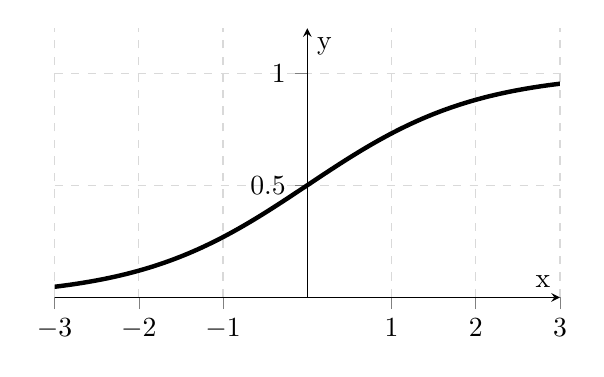
\begin{tikzpicture}
      \begin{axis}[
        legend pos=north west,
          axis x line=middle,
          axis y line=middle,
          width=8cm,
          height=5cm,       
          % x tick label style={/pgf/number format/fixed,
          %                     /pgf/number format/fixed zerofill,
          %                     /pgf/number format/precision=1},
          % y tick label style={/pgf/number format/fixed,
          %                     /pgf/number format/fixed zerofill,
          %                     /pgf/number format/precision=1},
          grid = major,
          grid style={dashed, gray!30},
          xmin=-3,
          xmax= 3,
          ymin= 0,
          ymax= 1.2,
          xlabel=x,
          ylabel=y,
          tick align=outside,
          enlargelimits=false]
        \addplot[black, ultra thick,samples=500] {1/(1 + exp(-x))};
      \end{axis}
    \end{tikzpicture}
    \label{fig:test1}
  \end{minipage}%
  \begin{minipage}{.5\textwidth}
    \centering
    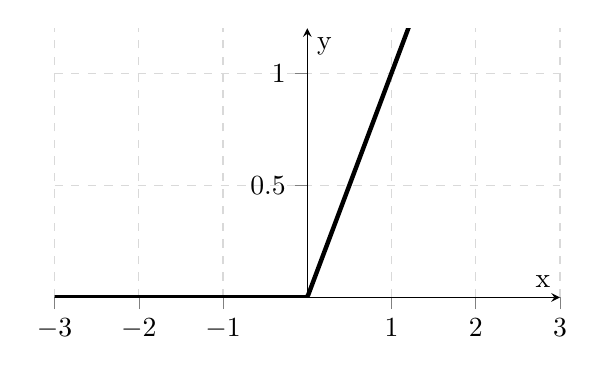
\begin{tikzpicture}
      \begin{axis}[
        legend pos=north west,
          axis x line=middle,
          axis y line=middle,
          width=8cm,
          height=5cm,
          % x tick label style={/pgf/number format/fixed,
          %                     /pgf/number format/fixed zerofill,
          %                     /pgf/number format/precision=1},
          % y tick label style={/pgf/number format/fixed,
          %                     /pgf/number format/fixed zerofill,
          %                     /pgf/number format/precision=1},
          grid = major,
          grid style={dashed, gray!30},
          xmin=-3,
          xmax= 3,
          ymin= 0,
          ymax= 1.2,
          xlabel=x,
          ylabel=y,
          tick align=outside,
          enlargelimits=false]
        \addplot[black, ultra thick,samples=500] {max(0, x))};
      \end{axis}
    \end{tikzpicture}
  \end{minipage}%
  \caption{The figure shows a plot of the hyperbolic  tangent  activation function on the left and a plot of the ReLU activation function on the right.}\label{fig:af}
\end{figure}


In order to avoid saturation problems, a commonly used non-linear activation function is the Rectified Linear Unit (ReLU) function \cite{Nair:2010:RLU:3104322.3104425}, which can be seen in figure \ref{fig:af}:\\

\begin{equation}
  \varphi(v) = \max(0, v)
\end{equation}
\\
ReLUs are non-saturating which results in a neuron always learning if the input is positive. Networks with ReLUs train several times faster and have become, as of 2015, the standard activation function for deep neural networks \cite{lecun2015deep}.

\subsection{Feedforward neural networks}
A feedforward neural network, or multilayer perceptron (MLP), is an ANN which consists of multiple layers $L$ of artificial neurons. The goal of a feedforward network, as to other Ml algorithms, is to approximate some function $\hat f$ \cite{Goodfellow-et-al-2016}. In terms of a classifier, $y= \hat f(x)$ maps an input $x$ to a label $y$. Consequently, a neural network with $m$ input nodes and 1 output node serves as a function with m inputs and 1 output.

\begin{figure}[h]
  \centering
  \def\layersep{3cm}
	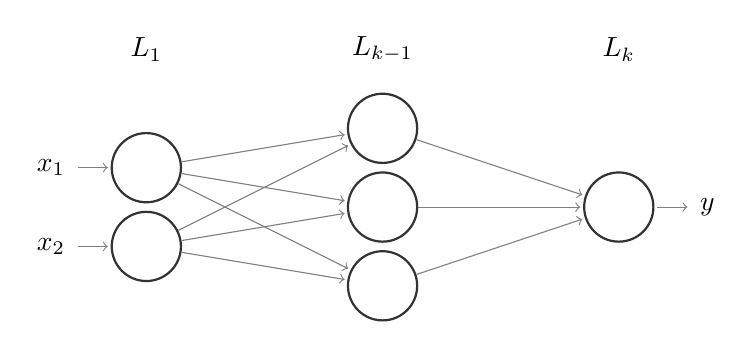
\begin{tikzpicture}[shorten >=1pt,->,draw=black!50, node distance=\layersep]
    \tikzstyle{every pin edge}=[<-,shorten <=1pt]
    \tikzstyle{neuron}=[circle,draw=black!80, thick,minimum size=25pt,inner sep=0pt]
    \tikzstyle{input neuron}=[neuron];
    \tikzstyle{output neuron}=[neuron];
    \tikzstyle{hidden neuron}=[neuron];
    \tikzstyle{annot} = [text width=4em, text centered]

    % Draw the input layer nodes
    \foreach \name / \y in {1,...,2}
    % This is the same as writing \foreach \name / \y in {1/1,2/2,3/3,4/4}
        \node[input neuron, pin=left:$x_{\y}$] (I-\name) at (0,-\y) {};

    % Draw the hidden layer nodes
    \foreach \name / \y in {1,...,3}
        \path[yshift=0.5cm]
            node[hidden neuron] (H-\name) at (\layersep,-\y cm) {};

    % Draw the output layer node
    \node[output neuron,pin={[pin edge={->}]right:$y$}, right of=H-2] (O) {};

    % Connect every node in the input layer with every node in the
    % hidden layer.
    \foreach \source in {1,...,2}
        \foreach \dest in {1,...,3}
            \path (I-\source) edge (H-\dest);

    % Connect every node in the hidden layer with the output layer
    \foreach \source in {1,...,3}
        \path (H-\source) edge (O);

    % Annotate the layers
    \node[annot,above of=H-1, node distance=1cm] (hl) {$L_{k-1}$};
    \node[annot,left of=hl] {$L_1$};
    \node[annot,right of=hl] {$L_k$};
\end{tikzpicture}
\caption{The diagram shows the typical structure of a feedforward network. The network has two input units in the input layer $L_1$ and one output unit in the output layer $L_k$. Layers $L_{2} \dots L_{k-1}$ the the so-called hidden layers.}\label{fig:ffnn}
\end{figure}
The network is named feedforward as it the information flowing through the network passes with the outermost input layer and and ends at the output unit of the output layer \cite{Goodfellow-et-al-2016}. All units in a layer are fully connected to the succeeding layer, however, there is no interconnection between units in the same layer. Figure \ref{fig:ffnn} shows a typical feedforward architecture with three layers including a single hidden layer $L_{k-1}$.\\

Considering equation \ref{eqn:neuron1}, we can now compute the input to the output node, given by\\
\begin{equation}
  \sum_{k=1}^{n} \alpha_k h_k
\end{equation}
\\
where $h_k$ is the output of the $k$th hidden node and $\alpha_k$ being the weight from the $k$th hidden to the output node. The output unit's activation function is then applied to this value, transforming the output to the given equation

\begin{equation}
  y = \varphi\left(\sum_{k=1}^{n} \alpha_k \varphi \left(\sum_{i=1}^{m} w_{ik} x_i + b \right)\right).
\end{equation}.

\subsection{Backpropagation}
\label{sec:backprop}
The purpose of the backpropagation algorithm \cite{rumelhart1988learning} is to adjust the synaptic weights of the network to approximate the function $\hat f$ mapping the inputs $x$ of the training data to the corresponding output labels $y$. In an iterative process the algorithm computes the overall error of the functional mapping and adjusts the weights of each neuron according to it's individual error contribution. The result of this algorithm is a neural network configured to sensibly respond to unseen inputs for the specific supervised learning task.

As a first step, the weights of the network are initialized which is usally done in a randomly manner or based on a certain heuristic. Then, each input pattern $p$, with features $p = \{x_0,x_1, x_2, \dots, x_n \}$ and label $y$, is then sequentially processed, layer by layer, by the network in two phases. In the first phase, the \textit{forward phase}, the ouput of the network is computed. The square error for the output nodes j is then calculated as follows, where $\hat{y}_j$ denotes the output node's generated output and $y_j$ is the desired ouput (see \cite{Haykin:1998:NNC:521706}):

\begin{equation}
  E = \frac{1}{2}\sum_{j} (\hat{y}_j - y_j)^2.
\end{equation}

Continuing in the \textit{backward phase}, the network measures how much each neuron in the output layer $L_k$ has contributed to each output neuron's error. Furthermore, as to measure the error contributions coming from each neuron in the previous layer, this step is repeated until the input layer is reached and all error contributions, the gradients, are computed. To put this in other words, the \textit{backwards phase} measures the error gradients across all connection weights in the network by propagating the error gradients back into the network.

In this iterative process, the error gradients of the error function are calculated based on the partial derivative with respect to each connecting weight. If we define $o_j$ as output of a neural unit with
\begin{equation}
  o_j = \varphi(net_j)
\end{equation}
and the units input as
\begin{equation}
  net_j = \sum_{j=1}^{n}x_{i}w_{ij},
\end{equation}
the chain rule can be applied in order to compute the partial derivatives as follows:

\begin{equation}
  \frac{\delta E}{\delta w_{ij}} = \frac{\delta E}{\delta o_j} \frac{\delta o_j}{\delta net_j} \frac{\delta net_j}{\delta w_{ij}}
\end{equation}

Given the partial derivative in respect to the weight $w_{ij}$, the change of the weight $\Delta w_{ij}$ can be determined. Here, the weight update equation (3.22) is computed depending on two cases. Either if the node $j$ is in the hidden layer or in the output layer:

\begin{equation}
  \Delta w_{ij} = -\eta \frac{\delta E}{\delta w_{ij}} = - \eta \delta_j o_i
\end{equation}

\begin{equation}
  \delta_j =
  \begin{cases}
    \varphi'(net_j)(o_j - \hat{y}_j) & \text{node $j \in L_k$}\\
    \varphi'(net_j) \sum_k \delta_k w_{jk} & \text{node $j \notin L_k$}
  \end{cases}
\end{equation}

In equation (3.23), $\eta$ denotes the \textit{learning rate}, which defines to which amount the reverse gradients are applied to the weight update; $k$ refers to a node in the successor layer of the node $j$.

Once the weights are updated, the global error of the network is calculated and the forward and the backward phase are repeated for the rest of the training patterns. One pass through all of the training patterns is called a \textit{training epoch}. Several strategies exist to stopping the described training process. One condition is to stop after to a fixed number of training epoches, a second can be a stop once the change in the weights reaches a certain low-end threshhold \cite{Haykin:1998:NNC:521706}. After the process, the final values of the weights are saved and can be used for prediting new incoming patterns.

% \subsection{Recurrent Neural Networks}
% In the previous section, we have looked at feedforward neural networks where information, as the name implies, flows only in one direction, from the input layer to the output layer. A recurrent neural network (RNN) is similar to a feedforward network, except that it also has cyclic connections. This structure makes a RNN able to memorize previous information that has flown throw the network.\\

% For each timestep $t$, the recurrent neuron, as illustrated in Figure bla, recieves the input $x_{(t)}$ as well as it's own ouput from the the previously compututed time step $y_{(t_{-1})}$. The network can then be transformed to represent the time axis, as illustrated in Figure bla, which is also refered to as \textit{unrolling through time}.\\

% In comparison to the feedforward neuron, the recurrent neuron has a pair of wights: one represents the inputs $x_{(t)}$ and the other for the ouput of the previous step $y_{(t_{-1})}$. We can define these weight vectors as $w_x$ and $w_y$. The output of a recurrent neuron can then be computed with following equation:\\

% \begin{equation}
% y(t) = \varphi \left( x_{(t)}^T  w_{x} + y_{t-1}^T  w_y + b \right)
% \end{equation}
% \\
% where $b$ refers to the \textit{bias} of the node.

% \subsection{Long-short term memory}
% As the RNN gains it's possibility to remember because of the recurrent neuron \textit{recurrent connection}, in practise, RNNs can forget patterns after a small amount of steps. Therefore, it is hard to train a RNN to identifiy time correlations of longer sequences. As we will be analyzing the time series data produced from the sensor components of the smartphone, I would like to introduce a varient of the RNN, called Long Short-Term Memory (LSTM).

% \begin{figure}
%   \centering
%   \begin{tikzpicture}[
%     prod/.style={circle, draw, inner sep=0pt},
%     ct/.style={circle, draw, inner sep=5pt, ultra thick, minimum width=10mm},
%     ft/.style={circle, draw, minimum width=8mm, inner sep=1pt},
%     filter/.style={circle, draw, minimum width=7mm, inner sep=3pt},
%     mylabel/.style={font=\scriptsize\sffamily},
%     >=LaTeX
%     ]

% \node[ct, label={[mylabel]Cell}] (ct) {$c_t$};
% \node[filter, right=of ct] (int1) {$\varphi$};
% \node[prod, right=of int1] (x1) {$\times$}; 
% \node[right=of x1] (ht) {$h_t$};
% \node[prod, left=of ct] (x2) {$\times$}; 
% \node[filter, left=of x2] (int2) {$\varphi$};
% \node[prod, below=5mm of ct] (x3) {$\times$}; 
% \node[ft, below=5mm of x3, label={[mylabel]right:Forget Gate}] (ft) {$f_t$};
% \node[ft, above=of x2, label={[mylabel]left:Input Gate}] (it) {$i_t$};
% \node[ft, above=of x1, label={[mylabel]left:Output Gate}] (ot) {$o_t$};

% \foreach \i/\j in {int2/x2, x2/ct, ct/int1, int1/x1,
%             x1/ht, it/x2, ct/it, ct/ot, ot/x1, ft/x3}
%     \draw[->] (\i)--(\j);

% \draw[->] (ct) to[bend right=45] (ft);

% \draw[->] (ct) to[bend right=30] (x3);
% \draw[->] (x3) to[bend right=30] (ct);

% \node[fit=(int2) (it) (ot) (ft), draw, inner sep=0pt] (fit) {};

% \draw[<-] (fit.west|-int2) coordinate (aux)--++(180:7mm) node[left]{$x_t$};
% \draw[<-] ([yshift=1mm]aux)--++(135:7mm);
% \draw[<-] ([yshift=-1mm]aux)--++(-135:7mm);

% \draw[<-] (fit.north-|it) coordinate (aux)--++(90:7mm) node[above]{$x_t$};
% \draw[<-] ([xshift=1mm]aux)--++(45:7mm);
% \draw[<-] ([xshift=-1mm]aux)--++(135:7mm);

% \draw[<-] (fit.north-|ot) coordinate (aux)--++(90:7mm) node[above]{$x_t$};
% \draw[<-] ([xshift=1mm]aux)--++(45:7mm);
% \draw[<-] ([xshift=-1mm]aux)--++(135:7mm);

% \draw[<-] (fit.south-|ft) coordinate (aux)--++(-90:7mm) node[below]{$x_t$};
% \draw[<-] ([xshift=1mm]aux)--++(-45:7mm);
% \draw[<-] ([xshift=-1mm]aux)--++(-135:7mm);
% \end{tikzpicture}
% \caption{The figure shows a LSTM cell.}
% \end{figure}
